% Copyright (c) 2023-2026 Oriol Cayon, Delft University of Technology
% SPDX-License-Identifier: Apache-2.0
%
% Numbers, tables and figures come from generated/ and figures/, written by
%   python scripts/reduced-order-model/optimization/cycle/report_cycle_optimisation.py
% Rebuild:  latexmk -pdf cycle_optimisation.tex   (in docs/cycle_optimisation/)
\documentclass[11pt,a4paper]{article}

\usepackage[margin=2.4cm]{geometry}
\usepackage{graphicx}
\usepackage{amsmath,amssymb}
\usepackage{booktabs}
\usepackage{xcolor}
\usepackage{caption}
\usepackage{subcaption}
\usepackage{float}
\usepackage{enumitem}
\usepackage{fancyhdr}
\usepackage{xurl}
\usepackage[hidelinks]{hyperref}
\usepackage{siunitx}
\usepackage{tikz}
\usetikzlibrary{positioning,arrows.meta,fit,backgrounds}
\sisetup{range-phrase={--},range-units=single}

\graphicspath{{figures/}}
% GENERATED by scripts/reduced-order-model/optimization/cycle/report_cycle_optimisation.py
\newcommand{\kiteName}{LEI-V3-KITE}
\newcommand{\seedRzero}{236.7}
\newcommand{\seedReeloutFraction}{0.65}
\newcommand{\seedBetaZeroDeg}{20}
\newcommand{\seedBetaAmpDeg}{5.7}
\newcommand{\seedAzAmpDeg}{17.2}
\newcommand{\seedBetaPeakDeg}{68.8}
\newcommand{\seedRampFraction}{0.49}
\newcommand{\seedAzReelinDeg}{20.6}
\newcommand{\seedHandoverPhase}{0.5}
\newcommand{\curvatureLimit}{0.08}
\newcommand{\curvatureRadius}{12.5}
\newcommand{\closureTol}{10}
\newcommand{\steerSlack}{0.05}
\newcommand{\autoMaxIter}{12}
\newcommand{\nodesPerSecond}{3}
\newcommand{\mPerFigure}{10}
\newcommand{\mReelinWindow}{15}
\newcommand{\trustMain}{0.05}
\newcommand{\trustPolish}{0.005}
\newcommand{\boxSpline}{0.15}
\newcommand{\boxRzero}{50}
\newcommand{\maxIter}{1000}
\newcommand{\limSteer}{0.175}
\newcommand{\limSteerRate}{0.145}
\newcommand{\limDepowerRate}{0.2}
\newcommand{\limVrMin}{-8}
\newcommand{\limVrMax}{3.5}
\newcommand{\limWinchAcc}{4}
\newcommand{\limAoaMaxDeg}{14}
\newcommand{\limHeightMin}{50}
\newcommand{\limRzeroMin}{180}
\newcommand{\limRzeroMax}{300}
\newcommand{\limBetaCoeffMaxDeg}{80}
\newcommand{\windRef}{6}
\newcommand{\windHeight}{6}
\newcommand{\windLaw}{explog}
\newcommand{\lobeM}{60}
\newcommand{\lobeKappaSketch}{0.121}
\newcommand{\lobeKappaDesigned}{0.078}
\newcommand{\lobeKappaFaired}{0.078}
\newcommand{\lobeDesignFreed}{17}
\newcommand{\lobeDesignMoveDeg}{2.1}
\newcommand{\lobePeakTargetDeg}{68.8}
\newcommand{\lobePeakAchievedDeg}{68.6}
\newcommand{\lobeFairTouched}{0}
\newcommand{\lobeFairMoveDeg}{0.00}
\newcommand{\dubinsHalves}{7}
\newcommand{\dubinsRadius}{60}
\newcommand{\dubinsRadiusDefault}{60}
\newcommand{\dubinsLength}{462}
\newcommand{\dubinsTurningDeg}{236}
\newcommand{\dubinsPieces}{6}
\newcommand{\dubinsApexDeg}{68.8}
\newcommand{\winchSlope}{5381}
\newcommand{\winchOffset}{0.412}
\newcommand{\winchGain}{-10.93}
\newcommand{\winchRef}{1.7}
\newcommand{\winchTmin}{865}
\newcommand{\winchTmax}{8400}
\newcommand{\upPowered}{1.7}
\newcommand{\upDepowered}{2.1}
\newcommand{\seedLobePower}{1.83}
\newcommand{\seedLobeDuration}{94.2}
\newcommand{\seedLobeClosure}{+14.5}
\newcommand{\seedLobeNodes}{283}
\newcommand{\seedLobeM}{60}
\newcommand{\seedLobeSteerMin}{-0.22}
\newcommand{\seedLobeSteerMax}{+0.19}
\newcommand{\seedLobeAoaMaxDeg}{7.4}
\newcommand{\seedLobeWallMin}{16}
\newcommand{\autoLobeMoves}{7}
\newcommand{\autoLobeStuck}{cannot close the cycle (gap +15.8 m) within knob ranges}
\newcommand{\seedDubinsPower}{1.78}
\newcommand{\seedDubinsDuration}{91.0}
\newcommand{\seedDubinsClosure}{+11.2}
\newcommand{\seedDubinsNodes}{275}
\newcommand{\seedDubinsM}{70}
\newcommand{\seedDubinsSteerMin}{-0.19}
\newcommand{\seedDubinsSteerMax}{+0.19}
\newcommand{\seedDubinsAoaMaxDeg}{7.1}
\newcommand{\seedDubinsWallMin}{5}
\newcommand{\archPower}{4.46}
\newcommand{\archEnergy}{0.31}
\newcommand{\archDuration}{68.6}
\newcommand{\archReeloutFraction}{0.72}
\newcommand{\archTensionMax}{5.95}
\newcommand{\archTensionMean}{4.42}
\newcommand{\archRmin}{215}
\newcommand{\archRmax}{286}
\newcommand{\archRzero}{241}
\newcommand{\archClosure}{0.00}
\newcommand{\archSteerMax}{0.35}
\newcommand{\archDepMin}{1.34}
\newcommand{\archDepMax}{2.10}
\newcommand{\archVrMin}{-5.0}
\newcommand{\archVrMax}{2.2}
\newcommand{\archM}{43}
\newcommand{\archNodes}{265}
\newcommand{\archFloorNodes}{62}
\newcommand{\archFloorReelin}{42}
\newcommand{\archSdotMax}{2.27}
\newcommand{\archSdotMedian}{0.0149}
\newcommand{\archSdotMaxS}{0.083}
\newcommand{\archTurnRadiusMin}{10.4}

\definecolor{accent}{HTML}{D55E00}
\definecolor{blue}{HTML}{0072B2}
\definecolor{green}{HTML}{009E73}
\captionsetup{font=small,labelfont=bf}
\setlist{itemsep=2pt,parsep=0pt,topsep=3pt}

\pagestyle{fancy}
\fancyhf{}
\fancyhead[L]{\small\textsc{AWETrim --- full-cycle optimisation}}
\fancyhead[R]{\small\thepage}
\renewcommand{\headrulewidth}{0.3pt}

\newcommand{\code}[1]{\texttt{\small #1}}
\newcommand{\vect}[1]{\boldsymbol{#1}}
\newcommand{\dd}{\mathrm{d}}

\title{%
  \vspace{-1.5cm}
  {\Huge\textbf{Full pumping-cycle optimisation}}\\[6pt]
  {\large One periodic path, one nonlinear program, and how to seed it}\\[10pt]
  {\normalsize Transcription, seed generation and staging, with LEI-V3 results}
}
\author{Oriol Cayon \\ \small Delft University of Technology}
\date{\today}

\begin{document}
\maketitle
\thispagestyle{fancy}

\begin{abstract}
\noindent
AWETrim optimises a whole pumping cycle of a soft kite (reel-out figure-eights,
the reel-in and both transitions) as \emph{one} periodic phase. The flight
path is a single periodic cubic B-spline on the sphere, the depower input is a
free per-node profile, the reel speed is a rate-limited control, and the
quasi-steady force balance of the reduced-order model (ROM) is imposed at every
node. The nonlinear program (NLP) that results is large, stiff and has a
nearly flat objective. Whether it converges depends almost entirely on the
initial guess. This note documents the transcription, and above all the
\emph{seed}: a synthetic cycle that is
trim-feasible at every node, closed in tether length, inside every bound
and under a curvature limit before the optimiser sees it. Two reel-in
constructions are described: a ``giant lobe'' of the figure-eight and a
designed Dubins path on the sphere. Both are followed by a spline design and
fairing step, a forward quasi-steady simulation and a rule-based tuner that
maps each symptom to the knob that relieves it. A proximal trust-region staging
then carries the seed to the optimum in one solve. Results for the LEI-V3
illustrate the pipeline.
\end{abstract}

\tableofcontents

%======================================================================
\section{Purpose and scope}

A pumping cycle has two phases with conflicting requirements. The reel-out flies
crosswind figure-eights at high tension; the reel-in depowers the kite, parks
it high in the wind window and pulls it back at low tension. The usual
treatment optimises them as separate phases joined by boundary conditions.
That needs a transition model and hand-chosen switching states, and it splits
the cycle-average power into two objectives that are coupled only through those
states. AWETrim instead writes the cycle as \emph{one} periodic phase:
\begin{itemize}
  \item the path is one periodic B-spline over the cycle, so the transitions
        are just parts of the path, with no switching states;
  \item depower $u_p(s)$ is a per-node decision over the whole cycle, so
        \emph{where} to depower is optimised, not prescribed;
  \item the reel speed $v_r$ is a control and the tether length closes
        exactly over the period.
\end{itemize}
The price is an NLP whose feasible set is narrow. At every node, the
quasi-steady trim must have a solution with steering and angle of attack
inside their bounds, and the shape of the path decides whether it does. The
objective, cycle-average power, is a flat ridge: many shapes give almost the
same power. Started from a careless guess, IPOPT either fails to find
a feasible point or slides along the ridge into a region where the trim no
longer exists. Most of the engineering is therefore in the \emph{seed},
and Sect.~\ref{sec:seed} is the core of this note.

The physics of the ROM is that of Cayon, van Deursen and
Schmehl~\cite{cayon2026rom}; the trajectory-optimisation framing follows
Cayon and Schmehl~\cite{cayon2026torque}. The code lives in
\path{scripts/reduced-order-model/optimization/cycle/}
(\code{fit\_periodic\_cycle\_config.py}, \code{run\_full\_cycle\_opti.py}) and
\path{src/awetrim/kinematics/parametrized_patterns.py} (path constructions,
spline design and fairing) and \path{src/awetrim/timeseries/phase_parametrized.py}
(the NLP transcription).

%======================================================================
\section{Problem formulation}
\label{sec:problem}

\subsection{Quasi-steady kite on a prescribed path}

The kite is a point mass at radius $r$, azimuth $\phi$ and elevation $\beta$
in the wind reference frame, flying in the course-aligned reference frame of
\cite{cayon2026rom}. The path is prescribed on the unit sphere by a path
parameter $s\in[0,1)$,
\begin{equation}
  \vect q(s) = \begin{pmatrix}\cos\phi(s)\cos\beta(s)\\ \sin\phi(s)\cos\beta(s)\\ \sin\beta(s)\end{pmatrix},
  \qquad \vect r = r\,\vect q(s),
\end{equation}
and the kite moves along it at rate $\dot s$. With the arc rate
$\sigma'(s)=|\vect q'(s)|=\sqrt{\beta'^2+\cos^2\!\beta\,\phi'^2}$, the
tangential speed and the course angle follow from the path alone,
\begin{equation}
  v_\tau = r\,\sigma'(s)\,\dot s, \qquad
  \chi = \operatorname{atan2}\!\left(\phi'\cos\beta,\ \beta'\right),
\end{equation}
and the course rate is $\dot\chi = k_g v_\tau/r$, with $k_g$ the geodesic
curvature of the path on the unit sphere. In the quasi-steady ROM the
tangential acceleration vanishes ($\dot v_\tau=0$) and the force balance in
the course frame,
\begin{equation}
  \vect F(\dot s,\,u_s,\,T,\,v_r,\,r,\,u_p;\ s) \;=\; m\vect a - \vect F_\mathrm{aero} - \vect F_\mathrm{tether} - \vect F_\mathrm{grav} = \vect 0 \in\mathbb R^3,
  \label{eq:trim}
\end{equation}
is a set of three algebraic equations at every point of the path. Given the
state $(s, r, v_r)$ and depower $u_p$, Eq.~\eqref{eq:trim} determines the speed
along the path $\dot s$, the steering $u_s$ that flies the prescribed course
rate, and the tether tension at the ground $T$. This is the \emph{trim}. A
path is flyable only if this root exists with $u_s$ and the angle of attack
$\alpha$ within bounds.

\paragraph{Curvature.}
The curvature of the path on the unit sphere is
$\kappa = |\vect q'\times\vect q''|/|\vect q'|^3$; it splits into a normal part
equal to one and the geodesic part, $\kappa^2 = 1 + k_g^2$. The physical
curvature of the flown path at radius $r$ is $\kappa/r$, and the turn radius is
$R=r/k_g$. Because the curvature limits used below correspond to radii of
\SIrange{12}{60}{m} at $r\approx\SI{240}{m}$ ($k_g\gtrsim 4$), $\kappa$ and
$k_g$ differ by less than \SI{3}{\percent} there.

\subsection{One periodic path for the whole cycle}

Azimuth and elevation are uniform periodic cubic B-splines with $M$ control
points each,
\begin{equation}
  \phi(s) = \sum_{j=0}^{M-1} C_{\phi,j}\, B_3\!\left(Ms - j\right),\qquad
  \beta(s) = \sum_{j=0}^{M-1} C_{\beta,j}\, B_3\!\left(Ms - j\right),
  \label{eq:spline}
\end{equation}
with the index of $B_3$ taken modulo $M$, so the path is $C^2$ and exactly
periodic in $s$. One period is one whole pumping cycle. The control points
$\vect C_\phi,\vect C_\beta$ are design variables, and their box bounds bound
the path through the convex-hull property. Each basis function is non-zero on
four knot intervals only, which the NLP exploits (Sect.~\ref{sec:numerics}).

\subsection{Winch}
\label{sec:winch}

Two winch descriptions are used, one in the forward simulation that builds
the seed and one in the NLP.

\paragraph{Force law (seed simulation).}
The forward simulation needs a closure for $v_r$. It uses a linear force law
whose zero-force reel speed shifts with depower,
\begin{equation}
  T = k\,\bigl(v_r - v_0(u_p)\bigr),\qquad
  v_0(u_p) = v_{00} + g\,(u_p - u_\mathrm{ref}),
  \label{eq:winch}
\end{equation}
softly clamped to $[T_{\min},T_{\max}]$ by a softplus/softminus pair of
sharpness $\num{e-3}$\,\si{N^{-1}}. With a negative gain $g$ the
\emph{same} law reels out when the kite is powered and reels in when it is
depowered (Fig.~\ref{fig:winch}); this is what lets a single phase march
through a whole cycle. On the LEI-V3 the law is regressed from the
2019-10-08 flight: $k=\SI{\winchSlope}{N\,s/m}$, $v_{00}=\SI{\winchOffset}{m/s}$,
$g=\SI{\winchGain}{m\,s^{-1}}$ per metre of power tape around
$u_\mathrm{ref}=\SI{\winchRef}{m}$, clamps
$[\num{\winchTmin},\num{\winchTmax}]$\,\si{N} (the upper clamp is the drum
rating from \code{system.yaml}).

\begin{figure}[H]
  \centering
  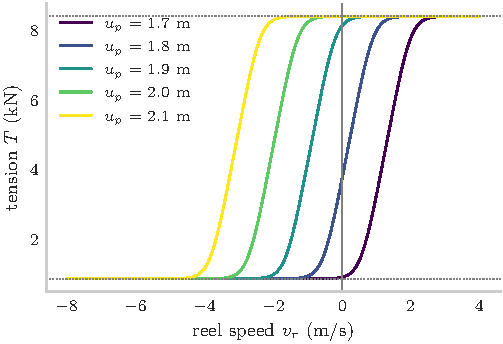
\includegraphics{winch_law.pdf}
  \caption{Depower-shifted winch law, Eq.~\eqref{eq:winch}, across the
  identified depower band $u_p\in[\upPowered,\upDepowered]$\,m (power-tape
  length). The same law holds the reel-out tension when powered and reels in
  when depowered. Dotted: soft clamps.}
  \label{fig:winch}
\end{figure}

\paragraph{Free reel speed (NLP).}
In the NLP the force law is dropped (\code{winch\_mode: free\_speed}). The reel
speed is a direct control, rate-limited by the drum acceleration
($|\dot v_r|\le\SI{\limWinchAcc}{m/s^2}$) and bounded to
$v_r\in[\limVrMin,\limVrMax]$\,\si{m/s}, and the tension is only required to
lie in the band the drum can hold, $T_{\min}\le T\le T_{\max}$. Keeping the
force law as an equality has two costs. Its soft clamp has $\partial T/\partial
v_r\approx 0$ on the plateau, which removes rank from the Jacobian exactly where
the optimum rides the force limit. It also ties radial closure to the tension
through a stiff relation. With free speed, closure is nearly linear in a direct
control. The optimal $T(v_r,u_p)$ relation is an \emph{output}, from which a
winch controller can be regressed afterwards (Fig.~\ref{fig:res-archived-power}).

\subsection{Transcription}

The cycle is discretised on $N$ nodes $s_i=i/N$. Per node the decisions are
\begin{equation}
  \vect x_i = \bigl(\dot s_i,\ u_{s,i},\ u_{p,i},\ v_{r,i},\ r_i,\ T_i\bigr),
  \qquad i=0,\dots,N-1,
\end{equation}
and the design parameters are $\vect p=(\vect C_\phi,\vect C_\beta,r_0)$, where
the operating radius $r_0$ is free within
\SIrange{\limRzeroMin}{\limRzeroMax}{m}.
Time follows from the path, $\Delta t_i=\Delta s/\dot s_i$ (left rule, the same
quadrature as the simulation), and the objective is the cycle-average
mechanical power
\begin{equation}
  \max_{\vect x,\vect p}\ \bar P = \frac{\sum_{i=0}^{N-2} T_i\, v_{r,i}\,\Delta t_i}{\sum_{i=0}^{N-2}\Delta t_i}.
  \label{eq:objective}
\end{equation}
Table~\ref{tab:constraints} lists the constraints. Two of them define the
cycle: the radial kinematics $r_{i+1}=r_i+v_{r,i}\Delta t_i$ and the hard
closure $r_{N-1}=r_0$. Closure must be an \emph{equality}. As a penalty it
lives in the objective, where it is exact only as its weight goes to
infinity, and the power reward for reeling out forever beats any finite
weight: the optimiser opens the cycle, the radius runs away and the trim
breaks.

\begin{table}[H]
  \centering\small
  \caption{Constraints of the full-cycle NLP (per node unless stated). Bounds
  are \code{DEFAULT\_OPTI\_LIMITS}, overlaid with the hardware limits of
  \code{system.yaml} and the seed's \code{opti\_limits\_override}; values are
  those of the LEI-V3.}
  \label{tab:constraints}
  \begin{tabular}{lll}
    \toprule
    constraint & expression & role \\
    \midrule
    trim & $\vect F(\vect x_i;\,s_i,\vect p)=\vect 0$ (3 rows) & Eq.~\eqref{eq:trim}, ROM \\
    radial kinematics & $r_{i+1}=r_i+v_{r,i}\,\Delta s/\dot s_i$ & tether length \\
    radius pin, closure & $r_0$ free, $r_{N-1}=r_0$ & periodic cycle \\
    winch band & $T_{\min}\le T_i\le T_{\max}$ & drum force rating \\
    reel speed & $\limVrMin\le v_{r,i}\le\limVrMax$\,\si{m/s} & drum speed range \\
    rate limits & $|\Delta u_s/\Delta t|\le\limSteerRate$\,\si{s^{-1}},
      $|\Delta u_p/\Delta t|\le\limDepowerRate$\,\si{m/s} & KCU \\
     & $|\Delta v_r/\Delta t|\le\limWinchAcc$\,\si{m/s^2} & drum \\
    steering & $|u_{s,i}|\le\limSteer$ & KCU range \\
    angle of attack & $0\le\alpha_i\le\limAoaMaxDeg^\circ$ & ROM validity \\
    height & $r_i\sin\beta(s_i)\ge\limHeightMin$\,\si{m} & safety \\
    path speed & $\dot s_i\ge 0.01$ & $\Delta t_i>0$ \\
    coefficients & $C_\beta\le\limBetaCoeffMaxDeg^\circ$, box on $C_\phi$ & convex hull \\
    turn radius (opt.) & $r_i\,\sigma'^3\ge R_{\min}|\kappa|\sigma'^3$, $\sigma'\ge0.2\,\bar\sigma'$ & 4 samples/interval \\
    \bottomrule
  \end{tabular}
\end{table}

The optional turn-radius constraint is written in polynomial form,
$-r\sigma'^3\le R_{\min}\,\kappa\sigma'^3\le r\sigma'^3$, rather than as
$R_{\min}|\kappa|\le r$. Near a forming cusp $\kappa\propto\sigma'^{-3}$ blows
up, and a cold solve that passes through such a shape stalls on the exploding
rows; the cross-product numerator stays bounded. It is enforced on four
sub-samples per interval because the spline can fold a cusp \emph{between}
two nodes, which no node-wise quantity sees. A floor on the arc rate keeps the
spline from ``hesitating'' ($\sigma'\to0$ over a sliver of $s$) to dodge it.

\subsection{What the seed must provide}
\label{sec:seedreq}

The NLP is solved with IPOPT from a primal warm start, the forward simulation
of the seed. Experience with this problem gives five requirements:
\begin{enumerate}
  \item \textbf{Trim everywhere.} Every node of the seed must trim. A node
        that fails leaves the per-node root problem without a nearby
        solution, and padding the warm start there breaks the NLP in ways
        that are hard to trace (\code{require\_full\_trajectory} aborts
        instead).
  \item \textbf{Inside the bounds.} Steering and angle of attack must stay within
        their bounds, so the active set at the start is the right one; a small
        steering overshoot (\num{\steerSlack}) is tolerated, because the flown
        KCU itself saturates at the bound and the NLP clips those nodes.
  \item \textbf{Closed.} $|r_\mathrm{end}-r_0|\le\SI{\closureTol}{m}$; an
        open seed starts the hard closure row far from feasible.
  \item \textbf{Smooth.} Path curvature under
        $\kappa_{\max}=\SI{\curvatureLimit}{m^{-1}}$ (radius
        \SI{\curvatureRadius}{m}). Sharp handovers between figures and reel-in
        show up as steering spikes the actuator cannot follow.
  \item \textbf{The right topology.} The optimiser can reshape the path, but
        it does not change the number of loops or the side of the reel-in
        reliably. Those choices belong to the seed.
\end{enumerate}
Section~\ref{sec:seed} constructs a seed that meets all five without any
flight data.

%======================================================================
\section{Seed generation}
\label{sec:seed}

\subsection{Overview}

Figure~\ref{fig:pipeline} summarises \code{fit\_periodic\_cycle\_config.py}.
Everything kite-specific comes from the kite's folder: hardware and actuator
ranges from \code{system.yaml}, the ROM and its identified depower band from
the ROM configuration, and wind, winch law and pattern size from
\code{cycle\_profile.yaml}. Nothing about a particular kite lives in the code.
The pipeline is geometric up to the forward simulation; only the tuning loop
costs simulations (about one minute each).

\begin{figure}[H]
\centering
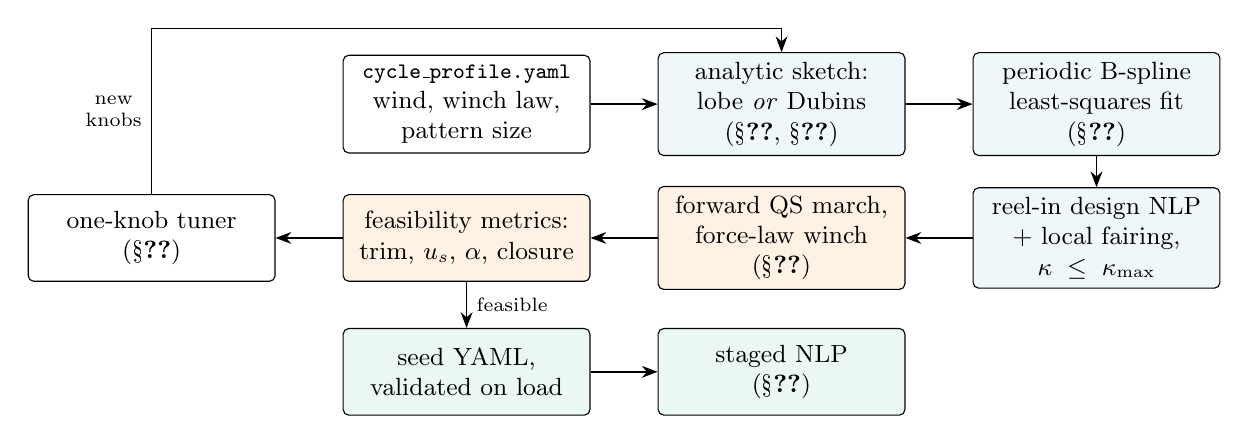
\begin{tikzpicture}[
  box/.style={draw, rounded corners=2pt, align=center, font=\small,
              minimum height=11mm, text width=29mm, fill=white},
  geo/.style={box, fill=blue!6},
  sim/.style={box, fill=orange!10},
  nlp/.style={box, fill=green!8},
  arr/.style={-{Stealth[length=2mm]}, semithick},
  lab/.style={font=\scriptsize, align=center}]
  % columns 0..3 at 40 mm, rows at 0 / -17 / -34 mm
  \node[box]  (prof)   at (40mm,0)    {{\footnotesize\texttt{cycle\_profile.yaml}}\\ wind, winch law,\\ pattern size};
  \node[geo]  (sketch) at (80mm,0)    {analytic sketch:\\ lobe \emph{or} Dubins\\ (\S\ref{sec:lobe}, \S\ref{sec:dubins})};
  \node[geo]  (fit)    at (120mm,0)   {periodic B-spline\\ least-squares fit\\ (\S\ref{sec:fit})};
  \node[box]  (tune)   at (0mm,-17mm) {one-knob tuner\\ (\S\ref{sec:auto})};
  \node[sim]  (check)  at (40mm,-17mm) {feasibility metrics:\\ trim, $u_s$, $\alpha$, closure};
  \node[sim]  (sim)    at (80mm,-17mm) {forward QS march,\\ force-law winch\\ (\S\ref{sec:forward})};
  \node[geo]  (design) at (120mm,-17mm) {reel-in design NLP\\ + local fairing,\\ $\kappa\le\kappa_{\max}$};
  \node[nlp]  (yaml)   at (40mm,-34mm) {seed YAML,\\ validated on load};
  \node[nlp]  (opt)    at (80mm,-34mm) {staged NLP\\ (\S\ref{sec:staging})};
  \draw[arr] (prof) -- (sketch);
  \draw[arr] (sketch) -- (fit);
  \draw[arr] (fit) -- (design);
  \draw[arr] (design) -- (sim);
  \draw[arr] (sim) -- (check);
  \draw[arr] (check) -- (tune);
  \draw[arr] (tune.north) |- node[pos=0.25, left, lab]{new\\knobs} ([yshift=3mm]sketch.north) -- (sketch.north);
  \draw[arr] (check) -- node[right, lab]{feasible} (yaml);
  \draw[arr] (yaml) -- (opt);
\end{tikzpicture}
\caption{Seed pipeline. Blue: pure geometry; orange: forward simulation;
green: written seed and the optimiser. An infeasible seed passes its
dominant symptom to the tuner, which moves one knob and rebuilds the sketch;
this loop runs only with \code{--auto}.}
\label{fig:pipeline}
\end{figure}

\subsection{The reel-in window and the synthetic depower}
\label{sec:window}

A fraction $f$ of the period is reel-out and the rest is reel-in. The reel-in
is a window of half-width $h=(1-f)/2$ centred at $s_c$, described by a smooth
bump $w(s)\in[0,1]$ built from Hermite smoothsteps
$S(x)=3x^2-2x^3$ on ramps of width $\rho(1-f)$:
\begin{equation}
  w(s) = S\!\left(\frac{d+h}{\rho(1-f)}\right)\Bigl[1-S\!\left(\frac{d-h+\rho(1-f)}{\rho(1-f)}\right)\Bigr],
  \qquad d = \bigl((s-s_c+\tfrac12)\bmod 1\bigr)-\tfrac12,
\end{equation}
with $S$ clamped to $[0,1]$. Measuring $d$ circularly lets the window wrap
across the periodic seam, so any centre is valid. The \emph{same} bump drives
the path shape and the synthetic depower,
\begin{equation}
  u_p(s) = u_{p,\mathrm{pow}} + \delta\, w(s)\,\bigl(u_{p,\mathrm{dep}}-u_{p,\mathrm{pow}}\bigr),
  \label{eq:depower}
\end{equation}
where $\delta\in(0,1]$ is the depower \emph{depth}. A mismatch between where
the kite is depowered and where it is flown high is a reliable way to
break the trim: a kite still powered while parked at \SI{70}{\degree}
elevation has no quasi-steady solution. The depth is the single radial-closure
knob. Through Eq.~\eqref{eq:winch} it sets the reel-in speed and therefore how
much tether comes back in.

\begin{figure}[H]
  \centering
  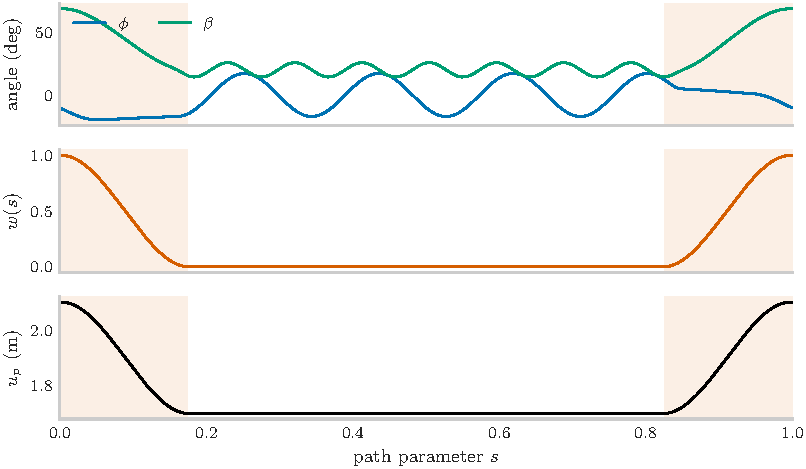
\includegraphics{seed_window.pdf}
  \caption{Lobe seed of the LEI-V3 over one period, at the default knobs
  ($f=\seedReeloutFraction$, ramp fraction $\rho=\seedRampFraction$,
  window centred at $s=0$, the top of the reel-in). Top: path angles; middle:
  the reel-in bump $w$; bottom: the synthetic depower profile,
  Eq.~\eqref{eq:depower}, with $\delta=1$. Shaded: reel-in window.}
  \label{fig:window}
\end{figure}

\subsection{Lobe reel-in: the cycle as one giant figure lobe}
\label{sec:lobe}

The first construction (\code{bow\_shape="lobe"}, the default) fades the
figure-eight out over the window and lifts the elevation:
\begin{align}
  \phi(s) &= \bigl(1-w\bigr)\,A\sin\psi(s) \;+\; w\,a\,b(\xi), \\
  \beta(s) &= \beta_0 + (\beta_\mathrm{pk}-\beta_0)\,w \;+\; \bigl(1-w\bigr)\,B\sin2\psi(s),
\end{align}
with figure amplitudes $A,B$, centre elevation $\beta_0$, reel-in peak
$\beta_\mathrm{pk}$, azimuth bow $a$ and $\xi\in[0,1]$ the position within the
window. Three details make this a feasible reel-in rather than a sketch:
\begin{description}
  \item[Frozen phase.] Over the first part of the entry ramp the figure rate
        $\dot\psi$ fades to zero with a smoothstep, so $\psi$ advances only a
        small budget (\SI{\seedHandoverPhase}{rad}) and then \emph{holds} through the window,
        resuming symmetrically on the exit ramp. The fading figure term is
        then a constant offset rather than a wiggle, and the climb peels off
        the last centre crossing in one clean arc. The figure-count residual
        that makes the phase exactly periodic is hidden in the plateau, where
        the figure amplitude is exactly zero.
  \item[Pinned handovers.] The frozen phases are pinned:
        $\psi_\mathrm{entry}=\pi-0.3$ (just before the climbing centre
        crossing) and $\psi_\mathrm{exit}=3\pi/2$ (the lobe extreme, heading
        down). The descent then lands \emph{tangentially} on a lobe and flies
        its lower half into the next crossing, so the reel-in replaces the top
        half of one lobe and slots into the alternation. The kite does not
        come down on a lobe that is already in progress.
  \item[One-sided bow.] The azimuth bow $b(\xi)$ rises over the last
        \SI{30}{\percent} of the entry ramp and does not return. Wherever the
        elevation plateau is flat, the azimuth must carry the path speed;
        a bow that stayed zero across the top would stall the parametrisation
        into a cusp.
\end{description}
\paragraph{Counting loops.}
With both phases pinned, the reel-out flies $n_\mathrm{ro}=k+\gamma$ figures,
where $k$ is an integer and $\gamma$ the fractional figure fixed by the
phase gap. The number of half-figures \emph{visible} during reel-out is
therefore $2n_\mathrm{ro}$, and its parity decides the re-entry side: odd counts
re-enter opposite the peel-off lobe, even counts on the same side. The
user-facing knob \code{--loops} is the visible count. The generator inverts the
snap and, when the requested parity does not match, moves the peel-off to the
mirrored climbing crossing ($\psi_\mathrm{entry}+\pi$) without touching the
landing. The one free topological choice is \code{--reelin smooth|cross}:
whether the top loop goes straight to the landing side or crosses the
ascending leg lower down.

\subsection{Dubins reel-in: a designed path on the sphere}
\label{sec:dubins}

The lobe shape fades one curve into another and inherits whatever curvature
the fade produces. The second construction (\code{--reelin dubins}) designs
the reel-in instead. The reel-out flies the plain figure
$\phi=A\sin\psi$, $\beta=\beta_0+B\sin2\psi$ from a landing at
$\psi=3\pi/2$ over a prescribed number of visible half-figures to a peel-off
state, and the reel-in joins the peel-off state (position \emph{and}
heading) to the landing state through a level apex at $\beta_\mathrm{pk}$.

\paragraph{Motion at bounded curvature on the sphere.}
Let $F=[\vect q,\vect t,\vect b]$ be the orthonormal frame of position,
heading and $\vect b=\vect q\times\vect t$. Per unit arc length on the unit
sphere, $\vect q'=\vect t$, $\vect t'=-\vect q+k\vect b$, $\vect b'=-k\vect t$,
i.e.\ $F' = F\,\hat{\vect\omega}$ with the constant axis $\vect\omega=(k,0,1)$.
A piece of constant geodesic curvature $k$ is therefore a rotation in closed
form (Rodrigues),
\begin{equation}
  F(\sigma) = F_0\,\exp\!\bigl(\sigma\hat{\vect\omega}\bigr)
  = F_0\Bigl[\mathbb I + \sin\theta\,\hat{\vect a} + (1-\cos\theta)\,\hat{\vect a}^2\Bigr],
  \qquad \vect a = \frac{\vect\omega}{|\vect\omega|},\ \theta=\sigma\sqrt{1+k^2},
\end{equation}
with $k=0$ a great circle. A turn of radius $R$ at $r_0$ has $k=r_0/R$.

\paragraph{Shortest legs.}
Each leg (peel-off$\to$apex, apex$\to$landing) is the shortest
arc--straight--arc (CSC) path between the two frames: arcs at $\pm k$, a
great circle between them, i.e.\ a Dubins path~\cite{dubins1957} on the
sphere~\cite{monroy1998}. The three lengths of each of the four types (LSL,
RSR, LSR, RSL) are found by multi-start least-squares shooting on the exact
motion; the shortest converged solution is kept per type.

\paragraph{Apex and radius are searched, not set.}
The apex azimuth is scanned over 25 values in
$\pm1.2|\phi_\mathrm{land}|$ and the shortest whole reel-in is kept. A
prescribed apex near the climb admits only paths with an extra loop, and at
high elevation a sideways metre is a lot of azimuth. Candidates that rise
above the apex or wrap behind the ground station are rejected. Radii from the
default \SI{\dubinsRadiusDefault}{m} down to the kite's turn-radius floor (or
half the default) are tried in steps of $\times0.85$. The reel-in with the
least \emph{total turning} wins, the larger radius on a tie, so a tighter
radius is used only where it saves a detour loop.

\paragraph{Timing.}
The reel-in occupies the window $u\in[f,1]$ of the period. Its path speed
eases from the figure speed at each end (over at most \SI{15}{\percent} of the
window) to a constant middle speed that covers the path length exactly, so
the curve is $C^1$ in $s$ and the periodic spline fits it without ringing.

\begin{figure}[H]
  \centering
  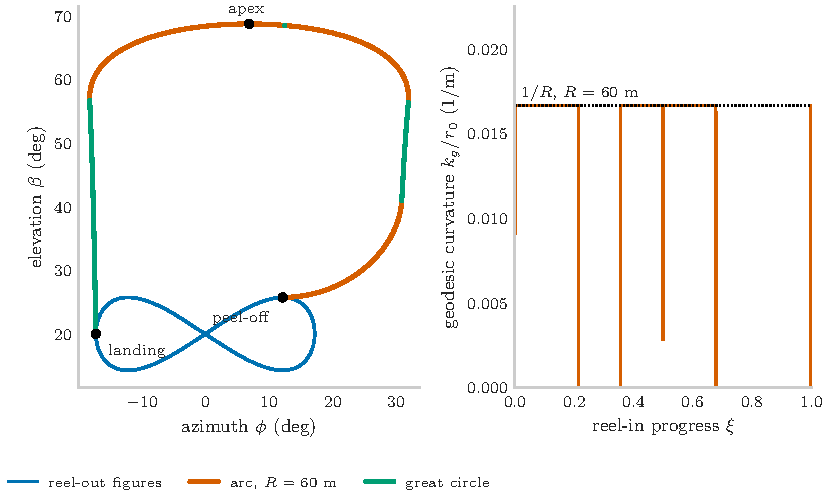
\includegraphics{seed_dubins.pdf}
  \caption{Dubins reel-in of the LEI-V3 seed, \dubinsHalves{} visible
  half-figures, apex at $\beta_\mathrm{pk}=\SI{\dubinsApexDeg}{\degree}$. Left:
  path in the wind window, reel-in coloured by piece. Right: geodesic
  curvature along the reel-in: arcs at $R=\SI{\dubinsRadius}{m}$, great
  circles at zero. The search keeps \dubinsPieces{} pieces (two CSC legs), a
  reel-in of \SI{\dubinsLength}{m} at $r_0=\SI{\seedRzero}{m}$.}
  \label{fig:dubins}
\end{figure}

\subsection{From sketch to spline}
\label{sec:fit}

\paragraph{Fit.}
The analytic sketch is sampled at 600 points and fitted by linear least
squares with the periodic basis of Eq.~\eqref{eq:spline}. The knots are uniform
in $s$, so the local resolution can only be set through $M$. The generator takes
\begin{equation}
  M = \max\!\Bigl(40,\ \bigl\lceil \mPerFigure\, n_\mathrm{loops}\bigr\rceil,\
      \bigl\lceil \mReelinWindow/(1-f)\bigr\rceil\Bigr),
\end{equation}
that is, at least \mPerFigure{} control points per figure-eight and \mReelinWindow{}
across the reel-in window. These are the measured knees of a convergence study
($\le$\SI{1}{m} path deviation at $r_0$). An under-resolved fit \emph{rings}:
the fitted spline's curvature can be several times that of the curve it fits.

\paragraph{Designing the reel-in.}
If the fitted spline violates $\kappa_{\max}$, the reel-in sketch is treated
as a drawing only, and the reel-in is designed between the two frozen handover
states. The control points whose whole support lies inside the window,
$\Delta\vect c$, solve
\begin{equation}
\begin{aligned}
  \min_{\Delta\vect c}\quad & \frac{\sum|\vect q''|^2}{E_{b,0}}
     + w_t\,\frac{\sum|\vect q'|^2}{E_{t,0}}
     + w_\mathrm{pk}\bigl(\beta(s_\mathrm{apex})-\beta_\mathrm{pk}\bigr)^2
     + w_\mathrm{tr}\,\frac{\sum|\Delta\phi|^2+|\Delta\beta|^2}{n\,(0.1)^2} \\
  \text{s.t.}\quad & \kappa^2\le(0.97\,\kappa_{\max} r_0)^2,\quad
     |\vect q'|^2\ge\tfrac14\min|\vect q'_0|^2,\quad |\Delta c|\le0.5,
\end{aligned}
\label{eq:design}
\end{equation}
with sums over a dense grid ($4000$ samples). The objective is a spline in
tension: bending energy plus a Dirichlet term ($w_t=1$). Without the tension
term, the minimum-bending way round a too-sharp corner is an outward teardrop
loop. The peak elevation is a target to hit ($w_\mathrm{pk}=100$), never a knob
that is quietly lowered. A weak tracking of the sketch ($w_\mathrm{tr}=0.1$)
holds the topology (which side, crossing or tangential). The window-edge
control points stay frozen, so the handover states and everything outside the
window are bit-identical, and $C^2$ continuity is automatic. The
curvature rows are normalised to $O(1)$ ($\kappa^2/(\cdot)^2-1\le0$) because the
raw form spans orders of magnitude across samples. The floor on $|\vect q'|$ prevents a
subtle failure: without it the solver satisfies the bound by stalling the
parametrisation between samples, and a forming cusp hides between grid
points.

\paragraph{Fairing.}
A residual pass catches anything outside the designed window (figures,
window edges). It finds the samples above $0.97\kappa_{\max}$ and frees
the control points supporting them plus one neighbour per side. It then
moves them by the \emph{least} amount, $\min|\Delta\vect c|^2$, under the
same curvature and arc-rate rows, inside a cumulative box of \SI{0.2}{rad}.
When a round fails it widens the freed set (up to five rounds). The box is
essential: from a badly violating start, IPOPT otherwise wanders into a
curvature-feasible but wildly deformed basin of giant loops.

\begin{figure}[H]
  \centering
  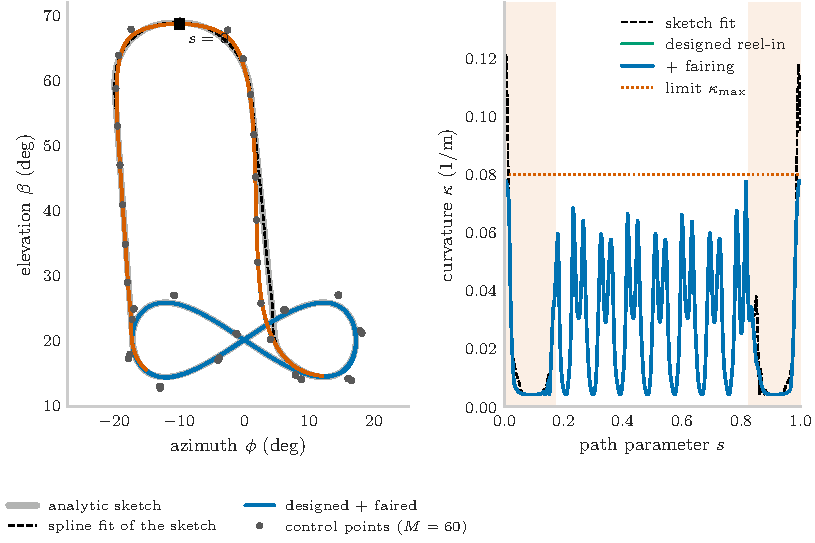
\includegraphics{seed_lobe.pdf}
  \caption{Lobe seed of the LEI-V3 at the default knobs ($M=\lobeM$). Left:
  analytic sketch, its spline fit, and the designed + faired spline (reel-in
  in orange). Right: curvature along the path. The fitted sketch peaks at
  \SI{\lobeKappaSketch}{m^{-1}} at the reel-in handovers; the reel-in design
  (\lobeDesignFreed{} control points) brings it to \SI{\lobeKappaDesigned}{m^{-1}}
  while hitting the peak elevation to within
  \SI{\lobePeakAchievedDeg}{\degree}/\SI{\lobePeakTargetDeg}{\degree} and moving
  the path by at most \SI{\lobeDesignMoveDeg}{\degree}. The fairing then has
  nothing left to do (\lobeFairTouched{} points moved).}
  \label{fig:lobe}
\end{figure}

\subsection{Forward simulation}
\label{sec:forward}

The geometric seed is then flown. The forward simulation marches node by
node along the spline. At each node it solves the trim, Eq.~\eqref{eq:trim},
together with the winch law, Eq.~\eqref{eq:winch}, for
$(\dot s,u_s,T,v_r)$ (a $4\times4$ root problem), and it integrates $r$ with
the same left rule as the NLP. Each node is seeded from the previous one,
with tiered fallback guesses when the first attempt fails. The march starts in
steady reel-out at the maximum tension and $r_0$. Its result is the NLP's warm
start, and it is reused for the first stage, so the optimiser does not repeat the
march. The measured cycle duration then sets the NLP grid,
$N=\lceil\nodesPerSecond\,T_\mathrm{cycle}\rceil$ nodes. The duration prior
in the profile can be off by a factor of two at other winds or loop counts.
In a convergence sweep, 3 nodes/s kept the cycle power within
\SI{0.2}{\percent} of a 400-node reference. At 2 nodes/s steering peaks fell
between nodes (the NLP only bounds nodes, so a coarse grid hides violations
rather than removing them), and at 1 node/s the trim broke.

\subsection{Automatic tuning}
\label{sec:auto}

With \code{--auto} the generator iterates
simulate~$\to$~metrics~$\to$~\emph{one} knob move. The metrics localise
each violation in $s$, and the location selects the lever:
\begin{itemize}
  \item a node that fails to trim is fixed first, in its region;
  \item angle-of-attack violations are always the slow top of the reel-in,
        where the kite is starved of apparent wind: lower $\beta_\mathrm{pk}$ by
        \SI{0.1}{rad};
  \item steering beyond the slack is handled according to where it occurs
        (Table~\ref{tab:levers});
  \item an open cycle is closed by the depower depth,
        $\delta\leftarrow\delta+\Delta r/(\SI{40}{m})$ (measured
        $\partial\Delta r/\partial\delta\approx\SI{-40}{m}$), and, once fully
        depowered, by shortening the reel-out fraction $f$.
\end{itemize}

\begin{table}[H]
  \centering\small
  \caption{Lever chains of the tuner by the region of the worst violation.
  A symptom that survives a move without improving the score by
  \SI{10}{\percent} escalates to the next lever in its chain.}
  \label{tab:levers}
  \begin{tabular}{lll}
    \toprule
    region & levers, in order & reason \\
    \midrule
    reel-in top & widen bow $|a|$ (+0.06 rad); lower $\beta_\mathrm{pk}$ & wider, faster arc at low wind \\
    reel-in edge & gentler ramp $\rho$; bigger figures; lower $\beta_\mathrm{pk}$ & handover sharpness \\
    figure-eights & bigger figures ($A\times1.12$, $B=A/2.5$) & turn rate $\sim4\pi/T_\mathrm{loop}$ \\
    \bottomrule
  \end{tabular}
\end{table}

The figure-eight lever comes from a simple estimate. A figure-eight sweeps the
course angle by $\pm2\pi$ per lobe, so at the kite's natural speed the steering
demand scales with the turn rate $4\pi/T_\mathrm{loop}$. The way to turn more
gently is a longer arc, i.e.\ bigger figures; azimuth and elevation amplitudes
are scaled together at $A\approx2.5B$. Each iterate is scored,
\begin{multline}
  \mathcal S = 100\,[\text{trim failed}]\Bigl(2-\frac{i_\mathrm{fail}}{N}\Bigr)
  + 50\,\max(\alpha-\alpha_{\max},0)
  + 10\max\bigl(|u_s|_{\max}-u_{s,\max}-\num{\steerSlack},0\bigr) \\
  + \frac{\max(|\Delta r|/\mathrm{m}-\closureTol,0)}{10}
  + 25\max\!\Bigl(\frac{\kappa_{\max}^\mathrm{spl}}{\kappa_{\max}}-1,0\Bigr),
\end{multline}
and the \emph{best} iterate is written, not the last (at most
\autoMaxIter{} iterations). The final knobs are printed so that they can be
pinned in \code{cycle\_profile.yaml} and reproduced without tuning.
Section~\ref{sec:results} shows a trace.

\subsection{Validation on load}

The optimiser re-checks the seed before solving and refuses it if it is
stale, hand-edited or assembled from mixed sources. The checks are: the
solver keys the generator writes are present; the depower profile has
$N+1$ entries inside the identified band; and no node in the top tenth of
the elevation range has a winch offset $v_0(u_p)>0$, i.e.\ the kite is never
commanded to reel out while parked high.

%======================================================================
\section{Optimisation strategy}
\label{sec:opt}

\subsection{Proximal staging}
\label{sec:staging}

The power objective is a flat ridge, and the periodic spline has near-null
re-parametrisation directions. Left free, IPOPT takes huge steps
($\|\vect d\|\sim10^2$) along them. Those steps merge or destroy figure-eight
loops and strand the iterate outside the trim-feasible region, where the
primal infeasibility explodes and never recovers. The solve is therefore
regularised with a proximal term on the design parameters,
\begin{equation}
  \min\ -\frac{\bar P}{P_\mathrm{s}} + w\sum_{p\in\vect p}\left(\frac{p-\hat p}{\Delta_p}\right)^2,
  \label{eq:proximal}
\end{equation}
where $\hat p$ is the warm-start value, $\Delta_p$ the width of the
parameter's bound and $P_\mathrm{s}$ the seed's average power. The quadratic
anchor adds curvature exactly in the null directions and so bounds the step,
while it barely resists directions with a real power gradient. A single solve
can therefore travel the whole way. Two stages are run
(Table~\ref{tab:stages}): a main stage with $w=\trustMain$, then a warm-started
polish with $w=\trustPolish$ that re-anchors at the main optimum and removes
most of the bias towards the seed. A hard box $|p-\hat p|\le\delta_p$ remains
as a backstop that should never bind; if it does, the driver warns and a
re-centred repeat pass (\code{--stage-repeats}) or a continuation
(\code{--continue-from}) is the remedy. After each stage a topology signature
(the number of prominent azimuth turns, about two per figure-eight plus the
reel-in) is compared with the seed's, and a change is reported even when
IPOPT reports success.

\begin{table}[H]
  \centering\small
  \caption{Stages of \code{run\_full\_cycle\_opti.py}. Both optimise
  $(\vect C_\phi,\vect C_\beta,r_0)$ and all per-node decisions under the hard
  closure; at most \maxIter{} IPOPT iterations each.}
  \label{tab:stages}
  \begin{tabular}{llll}
    \toprule
    stage & anchor $w$ & backstop box $\delta_p$ & IPOPT start \\
    \midrule
    main & \trustMain & $0.15$\,rad ($C$), \SI{\boxRzero}{m} ($r_0$) & cold barrier, seed primal \\
    polish & \trustPolish & $0.15$\,rad ($C$), \SI{100}{m} ($r_0$) & warm: $\mu_0=10^{-4}$, bound push $10^{-6}$ \\
    \bottomrule
  \end{tabular}
\end{table}

\subsection{Numerics}
\label{sec:numerics}

\begin{description}
  \item[Scaling.] Tension ($\sim10^3$--$10^4$\,N) and radius ($\sim10^2$\,m)
        are carried as $O(1)$ decisions divided by the 90th percentile of
        the warm start, and all equality rows are scaled likewise. Unscaled,
        the NLP oscillates and falls into restoration.
  \item[Local support.] A shared node function with symbolic $s$ references all
        $M$ control points and produces a dense $M$-wide Jacobian block per node.
        Instead, node functions are built per knot interval from a truncated
        copy of the spline that keeps only the four basis terms non-zero there.
        This is exact on that interval, and each node then couples to $4+4$
        control points. The Jacobian is about six times sparser, and
        whole-graph SX expansion costs about \SI{3.7}{MB} per node instead of
        \SI{24}{MB}.
  \item[Solver.] IPOPT with MUMPS and an L-BFGS Hessian, adaptive barrier,
        gradient-based scaling, \code{tol}$=10^{-5}$. L-BFGS floors the dual
        infeasibility at $10^{-2}$--$1$ on this problem, so the acceptable-point
        test is set to fire on feasibility alone (constraint violation
        $<10^{-4}$, objective change $<10^{-4}$ over five iterations).
\end{description}

%======================================================================
\section{Results for the LEI-V3}
\label{sec:results}

% Results of the full-cycle note; \input by cycle_optimisation.tex.
% Numbers are macros from generated/macros.tex.

All results are for the LEI-V3 with the flight-calibrated (semi-empirical)
ROM, at the wind of its \code{cycle\_profile.yaml}: an \windLaw{} profile with
\SI{\windRef}{m/s} at \SI{\windHeight}{m}. They come from two different code
states, which this section keeps apart:
\begin{itemize}
  \item \textbf{Seeds} (Sect.~\ref{sec:res-seeds}) were generated on
        2026-10-06 with the ROM rework later merged in PR~\#22 (standardised
        steering, bound $|u_s|\le\limSteer$; AoA bound
        \SI{\limAoaMaxDeg}{\degree}), still on the semi-empirical ROM, i.e.\
        before the aerostructural ROM became the LEI-V3 default.
  \item \textbf{The optimum} (Sect.~\ref{sec:res-opt}) is the last converged
        LEI-V3 full-cycle solve, from 2026-08-27, at the same wind. It
        predates the Dubins reel-in, the reel-in design step and the steering
        standardisation, so it is shown as an illustration of what the staged
        NLP does, not as a result of the code described above.
\end{itemize}
Sect.~\ref{sec:res-status} states why no fresh optimum is reported.

\subsection{Seed generation}
\label{sec:res-seeds}

Two seeds with \dubinsHalves{} visible half-figures were generated. The
\emph{lobe} seed used \code{--auto}, starting from the default knobs of
Fig.~\ref{fig:lobe}. The \emph{Dubins} seed used \code{--reelin dubins
--loops~7 --check}: no tuning, only the forward simulation and the grid
recalibration. Figure~\ref{fig:res-seeds} shows both paths and
Table~\ref{tab:seeds} summarises them.

\begin{figure}[H]
  \centering
  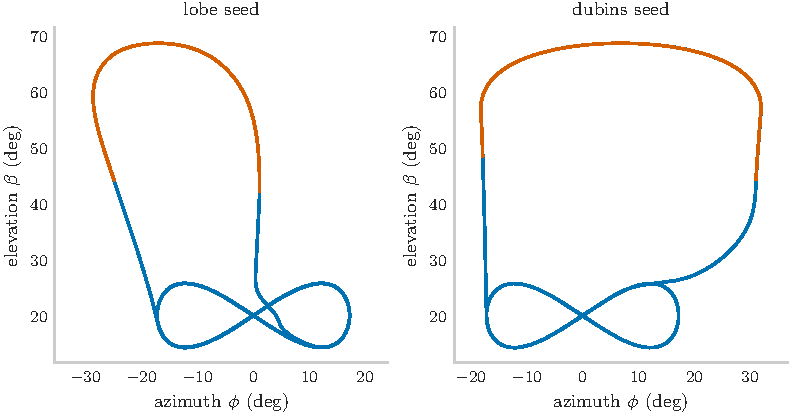
\includegraphics{results_seeds.pdf}
  \caption{The two generated LEI-V3 seeds in the wind window; reel-in (depower
  above mid-band) in orange. Left: lobe seed after \code{--auto}; right:
  Dubins seed.}
  \label{fig:res-seeds}
\end{figure}

\begin{table}[H]
  \centering\small
  \caption{Generated seeds and their forward simulations. Steering and AoA
  ranges are to be read against the NLP bounds $|u_s|\le\limSteer$ (plus
  the \num{\steerSlack} warm-start slack) and
  $\alpha\le\SI{\limAoaMaxDeg}{\degree}$; closure against
  \SI{\closureTol}{m}.}
  \label{tab:seeds}
  % GENERATED by report_cycle_optimisation.py
\begin{tabular}{lrr}
\toprule
quantity & lobe seed & dubins seed \\
\midrule
$M$ / $N$ & $60$ / $283$ & $70$ / $275$ \\
nodes trimmed & $283/283$ & $275/275$ \\
max curvature (1/m) & $0.077$ & $0.065$ \\
cycle duration (s) & $94.2$ & $91.0$ \\
average power (kW) & $1.83$ & $1.78$ \\
closure $r_\mathrm{end}-r_0$ (m) & $+14.5$ & $+11.2$ \\
$u_s$ range (-) & $-0.22$ / $+0.19$ & $-0.19$ / $+0.19$ \\
max $\alpha$ (deg) & $7.4$ & $7.1$ \\
max tension (kN) & $3.96$ & $3.95$ \\
tuner iterations & 8 & -- \\
generation time (min) & $16$ & $5$ \\
\bottomrule
\end{tabular}

\end{table}

\paragraph{What worked.}
Both seeds trim at every node of the recalibrated grid, stay under the
curvature limit, and keep the angle of attack inside its bound with a wide
margin. The Dubins seed reached this \emph{without any tuning}. Its
steering grazes the bound (\seedDubinsSteerMin{}/\seedDubinsSteerMax) by less
than the slack. The lobe seed needed the tuner (Table~\ref{tab:trace}), and
its first three moves are the case the lever chains were written for. The
steering violation sat at the top of the reel-in ($s\approx0.01$--$0.02$; the
window is centred on $s=0$), and widening the bow $|a|$ shrank it step by
step, from 31 violating nodes to 9.

\paragraph{What did not.}
Neither seed closes to within \SI{\closureTol}{m}: they end
\SI{\seedLobeClosure}{m} (lobe) and \SI{\seedDubinsClosure}{m} (Dubins) long.
For the lobe seed, the tuner's closure lever was already exhausted at full
depower depth, and its fallback, shortening the reel-out fraction from
0.65 to 0.53, moved the gap by less than a metre. The tuner therefore
stopped and wrote its best iterate (``\autoLobeStuck''). A closure that is
insensitive to the reel-in fraction means that the reel-in speed, and not
the reel-in duration, limits how much tether comes back. The reel-in speed
is set by the depower-shifted winch law of Eq.~\eqref{eq:winch}. On paper, a
\SIrange{11}{17}{m} gap on $r_0=\SI{\seedRzero}{m}$ is a small closure
residual that the NLP's first iterations can absorb (Sect.~\ref{sec:seedreq}).

\begin{table}[H]
  \centering\small
  \caption{\code{--auto} trace of the lobe seed: one knob per iteration,
  chosen from the dominant symptom and its location.}
  \label{tab:trace}
  % GENERATED by report_cycle_optimisation.py
\begin{tabular}{rp{0.5\textwidth}l}
\toprule
it. & dominant symptom & knob move \\
\midrule
1 & steering [-0.37, +0.19] at 31 node(s), worst at s=0.02 & az\_reelin\_amp $-0.36\to-0.42$ \\
2 & steering [-0.32, +0.19] at 12 node(s), worst at s=0.01 & az\_reelin\_amp $-0.42\to-0.48$ \\
3 & steering [-0.24, +0.19] at 9 node(s), worst at s=0.01 & az\_reelin\_amp $-0.48\to-0.54$ \\
4 & under-reel +14.9 m at full depower & reelout\_fraction $0.65\to0.61$ \\
5 & under-reel +14.8 m at full depower & reelout\_fraction $0.61\to0.57$ \\
6 & steering [-0.26, +0.18] at 9 node(s), worst at s=0.02 & az\_reelin\_amp $-0.54\to-0.60$ \\
7 & under-reel +14.5 m at full depower & reelout\_fraction $0.57\to0.53$ \\
8 & cannot close the cycle (gap +15.8 m) within knob ranges & stop, best iterate \\
\bottomrule
\end{tabular}

\end{table}

\begin{figure}[H]
  \centering
  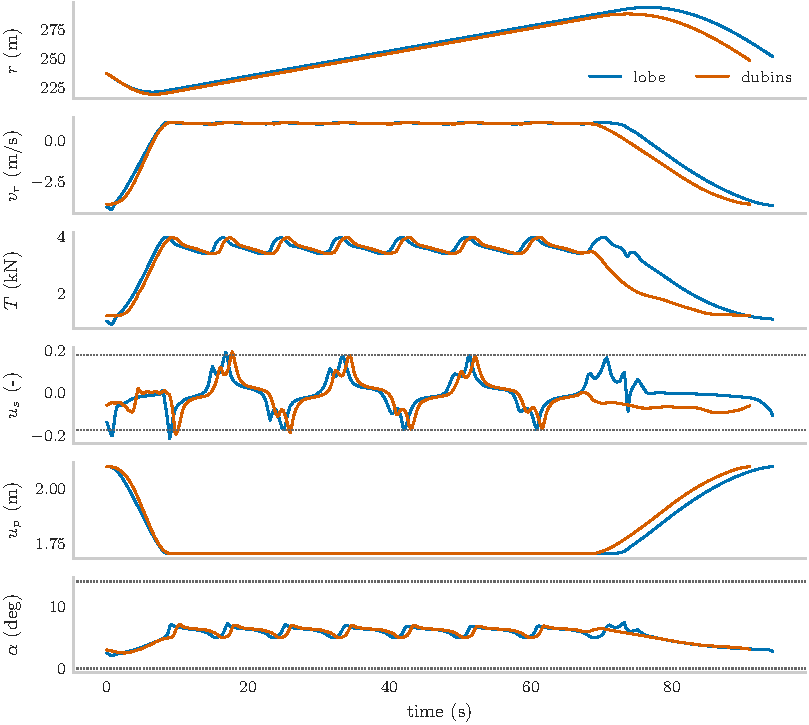
\includegraphics{results_seed_series.pdf}
  \caption{Forward simulations of the two seeds, which are the NLP warm
  starts. Dotted: NLP bounds on steering and angle of attack. Both cycles
  are about \SI{90}{s} long; the reel-in is the stretch of negative $v_r$ and
  high $u_p$.}
  \label{fig:res-seedseries}
\end{figure}

\subsection{An optimised cycle (2026-08-27)}
\label{sec:res-opt}

Figures~\ref{fig:res-archived-power} and~\ref{fig:res-archived} show the last
converged solve. The figure was written by that run itself and compares its
seed (a lobe seed of that time) with the optimum. The staged NLP raised the
cycle-average power from \SI{1.24}{kW} to \SI{\archPower}{kW} and shortened
the cycle to \SI{\archDuration}{s}, with the closure satisfied to
\SI{\archClosure}{m} and $r_0$ moved to \SI{\archRzero}{m}. The mechanisms
are visible in the per-node decisions:
\begin{itemize}
  \item \textbf{Reel-out at higher load.} The depower profile leaves the
        identified band towards the powered side ($u_p$ down to
        \SI{\archDepMin}{m}), and the tension rises to \SI{\archTensionMax}{kN}
        peak (\SI{\archTensionMean}{kN} mean), reeling out at up to
        \SI{\archVrMax}{m/s}.
  \item \textbf{Shorter, faster reel-in.} The reel speed reaches
        \SI{\archVrMin}{m/s}, and the reel-out time fraction of the cycle is
        \num{\archReeloutFraction}.
  \item \textbf{Free-speed winch.} The optimal $T(v_r)$ points do not lie
        on the flight-regressed force law the seed was marched with
        (Fig.~\ref{fig:res-archived-power}, bottom left). The regression of a
        controller from the optimum is a separate step.
\end{itemize}

\begin{figure}[H]
  \centering
  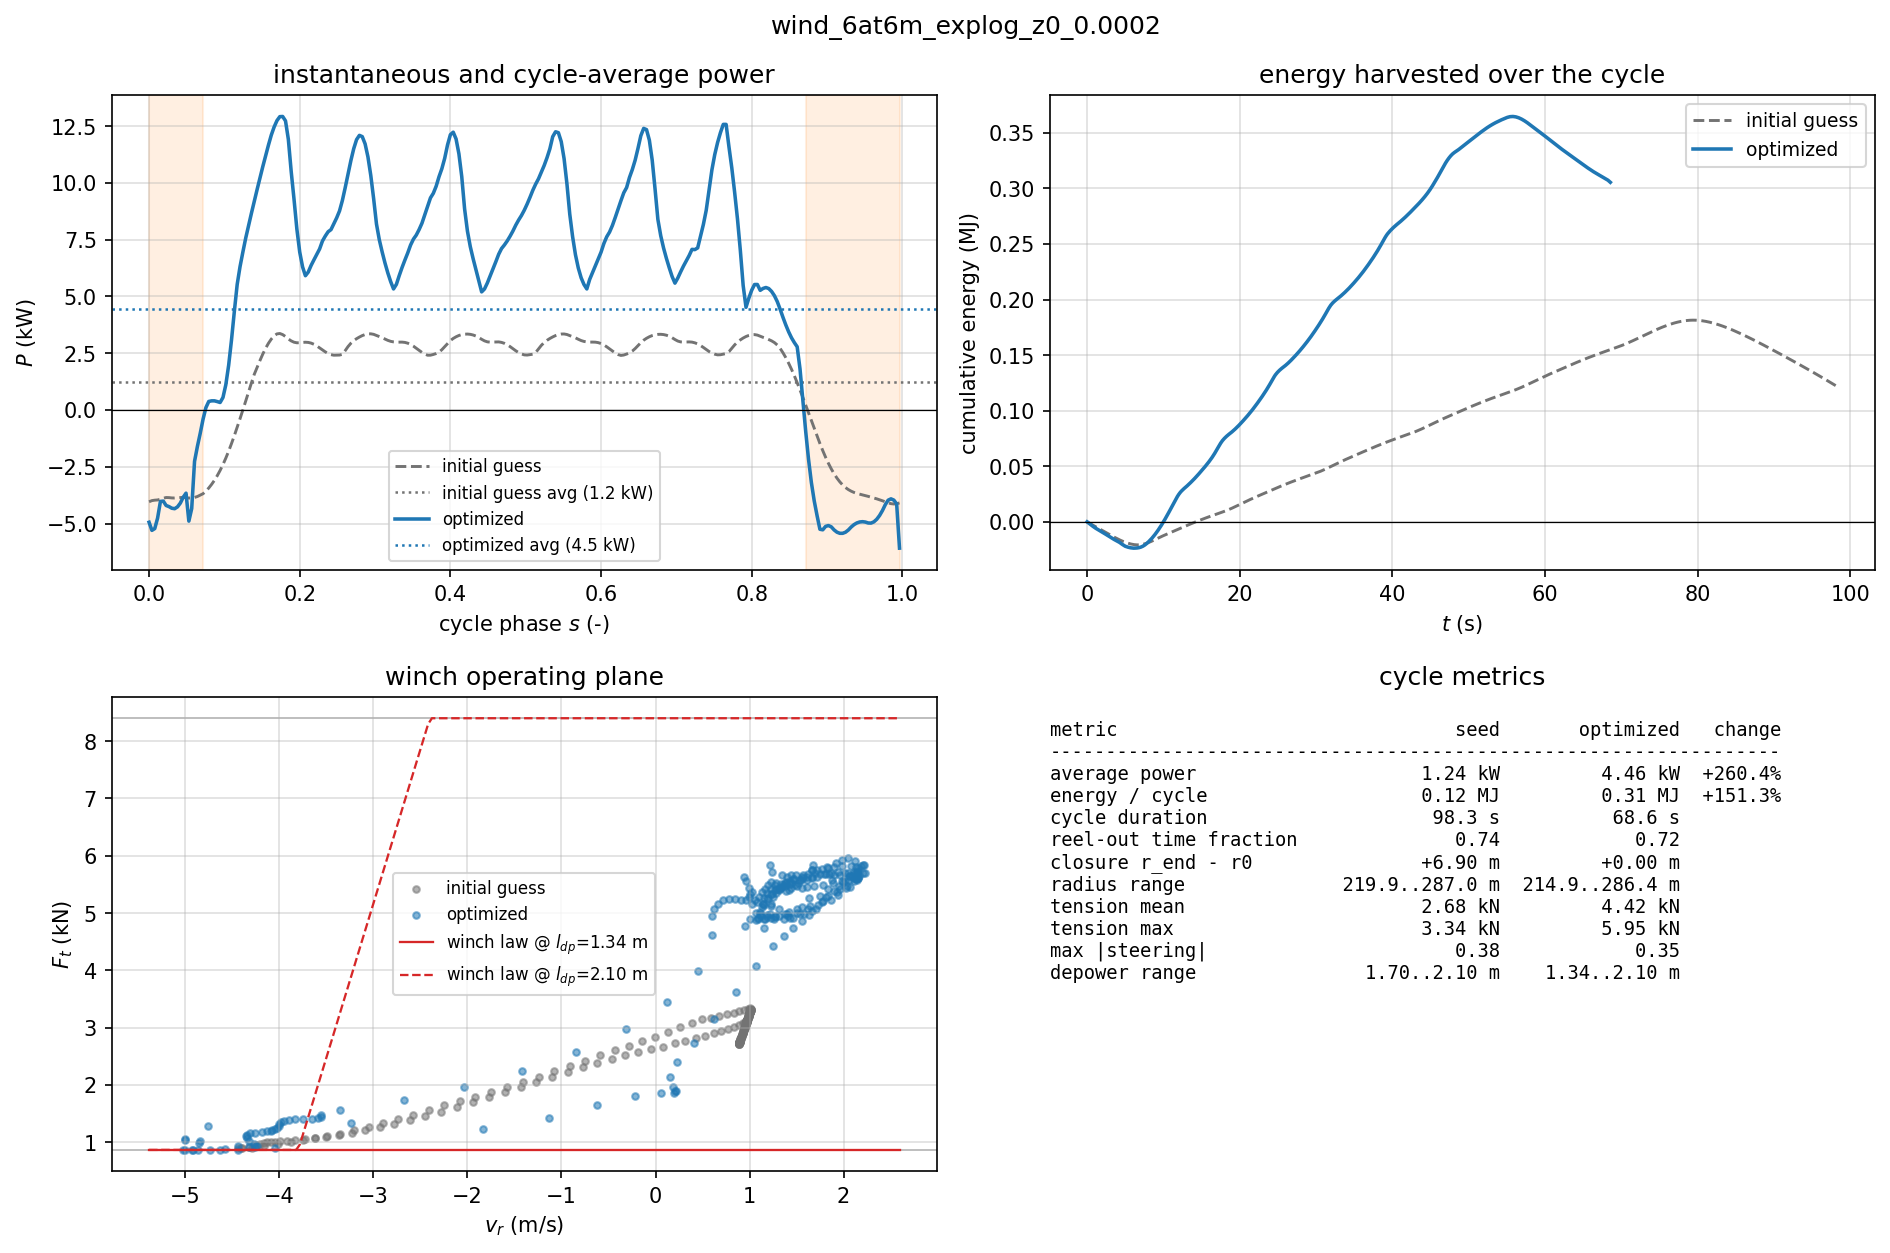
\includegraphics[width=\textwidth]{archived_power.png}
  \caption{Seed versus optimum of the 2026-08-27 LEI-V3 solve, as written by
  \code{run\_full\_cycle\_opti.py}: instantaneous and average power, cumulative
  energy, winch operating plane and metrics. Shaded: reel-in.}
  \label{fig:res-archived-power}
\end{figure}

\begin{figure}[H]
  \centering
  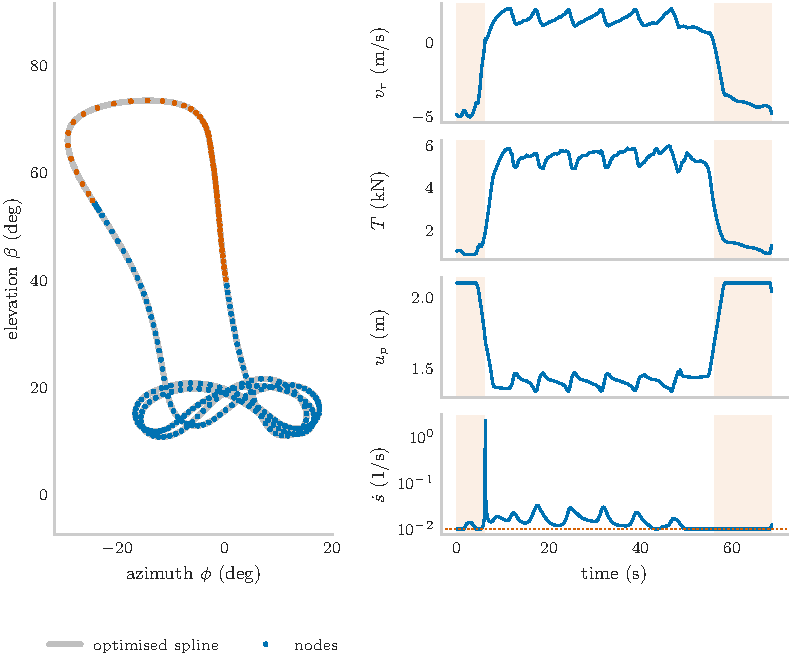
\includegraphics{results_archived.pdf}
  \caption{The 2026-08-27 optimum ($M=\archM$, $N=\archNodes$ nodes). Left:
  optimised spline and the node positions, reel-in ($v_r<0$) in orange.
  Right: reel speed, tension, depower and path rate $\dot s$; the dotted line
  is the numerical floor $\dot s\ge0.01$.}
  \label{fig:res-archived}
\end{figure}

\paragraph{Caveats of this optimum.}
Four features of the 2026-08-27 solution show what the constraints of that
time did not yet cover. Each motivated a later addition to the method:
\begin{enumerate}
  \item The depower profile goes down to \SI{\archDepMin}{m}, below the band
        $[\upPowered,\upDepowered]$\,m on which the ROM was identified, so
        the reel-out extrapolates the ROM. The band is now declared in the
        ROM file, and the AoA bound can be set from the ROM's validity range.
  \item The flown turn radius drops to \SI{\archTurnRadiusMin}{m}, because
        no turn-radius constraint existed. The optional sub-sampled
        constraint of Table~\ref{tab:constraints} was added for this.
  \item \archFloorNodes{} of the \archNodes{} nodes sit on the numerical
        floor $\dot s=0.01$: \archFloorReelin{} while reeling in, most of
        the rest in the transition into the reel-in (Fig.~\ref{fig:res-archived},
        bottom right). There the time step $\Delta t=\Delta s/\dot s$ is
        capped by a guard rather than set by the physics, so the reel-in
        timing of this optimum is partly an artefact of that bound.
  \item One node ($s=\archSdotMaxS$) has $\dot s=\SI{\archSdotMax}{s^{-1}}$,
        about 150 times the median \SI{\archSdotMedian}{s^{-1}}. Since
        $v_\tau=r\sigma'\dot s$ stays ordinary, the arc rate $\sigma'$ of the
        spline nearly vanishes there and $\dot s$ jumps to compensate, a
        \emph{hesitation point}. The floor $\sigma'\ge0.2\bar\sigma'$ that now
        comes with the turn-radius constraint
        (Table~\ref{tab:constraints}) excludes it.
\end{enumerate}
Its steering also reaches $|u_s|=\archSteerMax$, which was the steering bound
before the steering input was standardised.

\subsection{Status}
\label{sec:res-status}

With the code of 2026-10-06, both on commit \code{722488a} and with the ROM
rework of PR~\#22, the staged NLP does not converge for the LEI-V3 at this
wind. Started from the seeds above, the main stage stays close to feasible
(primal infeasibility \num{0.1}--\num{0.4}) for about 200 iterations, then
diverges and ends in restoration at the \maxIter-iteration cap. On the last
commit the seed itself is harder: the tuner lowered $\beta_\mathrm{pk}$ to
its floor without bringing the reel-in angle of attack inside its bound. Where
the regression since 2026-08-27 comes from (ROM, steering standardisation,
seed changes or staging) has not been isolated. Until it has, the seed
results of Sect.~\ref{sec:res-seeds} describe the current code, and the
optimum of Sect.~\ref{sec:res-opt} describes what the method produced when
it last converged.


%======================================================================
\section{Reproduction}

From the project root:
\begin{enumerate}
  \item \path{python scripts/reduced-order-model/optimization/cycle/fit_periodic_cycle_config.py --kite LEI-V3-KITE --auto}
        (lobe seed), or \code{--reelin dubins --loops 7 --check} (Dubins seed);
  \item \path{python scripts/reduced-order-model/optimization/cycle/run_full_cycle_opti.py --kite LEI-V3-KITE};
  \item \path{python scripts/reduced-order-model/optimization/cycle/report_cycle_optimisation.py --run lobe=<kite dir> --run dubins=<kite dir> --logs <dir>},
        then \code{latexmk -pdf} in \path{docs/cycle_optimisation/}.
\end{enumerate}
The seed is written to \path{<kite>/cycle_configs/full_cycle_periodic_from_exp.yaml}
and the optimum to \path{results/<kite folder>/optimization/full_cycle/}. To
keep the tracked LEI-V3 seed untouched, the runs of Sect.~\ref{sec:results}
were made on copies of the kite folder; \code{--kite} accepts any folder laid
out like \path{data/LEI-V3-KITE/}.

\begin{thebibliography}{9}
\bibitem{cayon2026rom}
O.~Cayon, V.~van~Deursen and R.~Schmehl,
\emph{Translational dynamics of bridled kites: a reduced-order model in the
course reference frame}, Wind Energ.\ Sci.\ 11, 1097--1121, 2026.

\bibitem{cayon2026torque}
O.~Cayon and R.~Schmehl, trajectory optimisation of soft-kite pumping cycles
with a quasi-steady reduced-order model, extended abstract,
The Science of Making Torque from Wind (TORQUE), 2026.

\bibitem{dubins1957}
L.~E.~Dubins,
\emph{On curves of minimal length with a constraint on average curvature, and
with prescribed initial and terminal positions and tangents},
Am.\ J.\ Math.\ 79, 497--516, 1957.

\bibitem{monroy1998}
F.~Monroy-P\'erez,
\emph{Non-Euclidean Dubins' problem},
J.\ Dyn.\ Control Syst.\ 4, 249--272, 1998.
\end{thebibliography}

\end{document}
